
%%% Local Variables: 
%%% mode: latex
%%% TeX-master: "russian"
%%% End: 

\section{使用glade}

Glade是一个程序界面设计工具,使用它你可以很方便的制作出各种界面。并且,在程序代码
中,不需要对界面进行定义和配置,大大缩短了程序开发周期。Glade将界面信息保存到一
个glade文件中,应用程序通过调用这个glade文件即可生成用户界面。

Glade设计初衷就是要把GTK+/GNOME程序的界面描述从源代码里分离出来,即使用xxx.glade
文件来描述界面,而不是把生成界面的c代码写再源代码中,这样的好处就是在后期修改程序
界面非常容易,你只需要使用Glade来调整界面即可(实际是仅仅修改了xxx.glade 文件,无
需对源程序做改动)。另外,使用glade文件来生程序界面并不会影响到你的程序的效率,因
为你只需要一次装入所有界面,然后在需要时直接使用。

在这里我们用glade对俄罗斯方块程序进行设计,首先画程序的草
图,见\pageref{fig:interface}页图\ref{fig:interface},主窗体由三部分组
成,上部``russian game''标题栏、底部``status''状态栏、中部游戏区,可由一
个GtkVBox组合起来;中部游戏区由两部分组成,左边``draw area''(显示区),右边控制
区,可由一个GtkHBox组合起来;右边控制区由三部分组成,依次是``next mass''(下一方
块)、``begin''按钮、``pause''按钮,可由一个GtkVBox组合起来。

\begin{figure}[htbp]
  \centering
  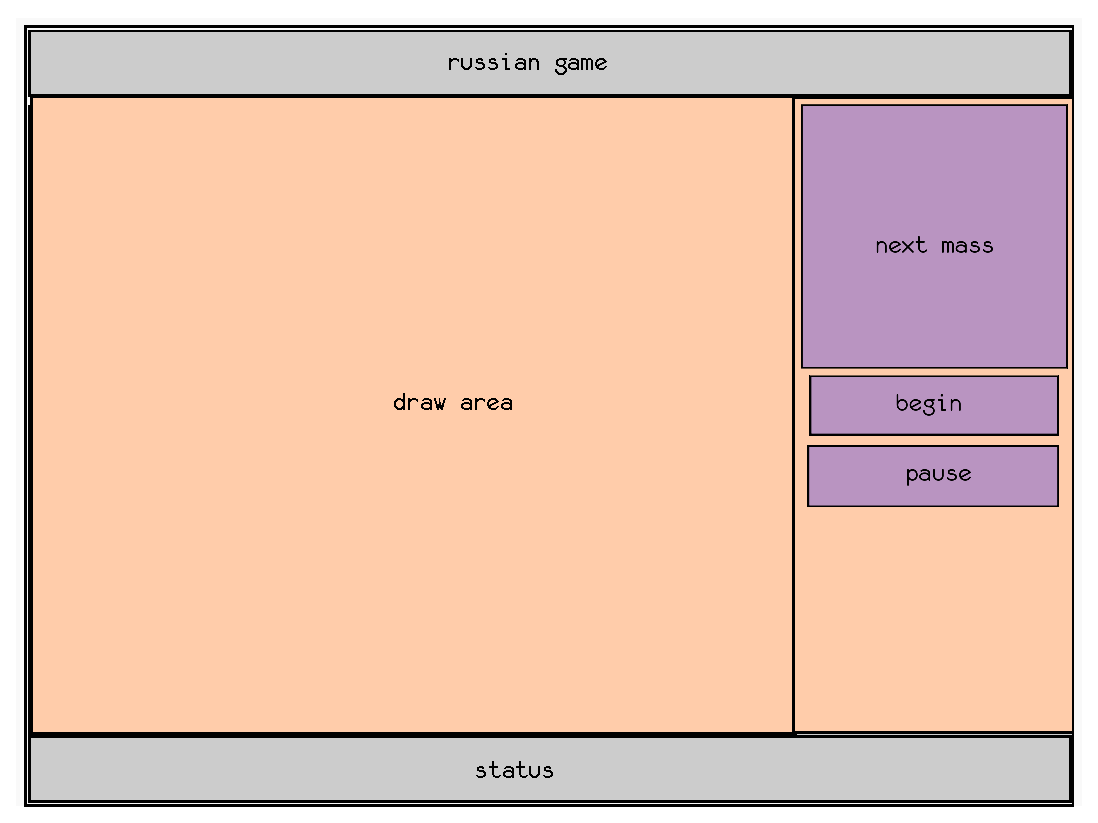
\includegraphics[width=3.5in]{images/interface}
  \caption{程序草图}
  \label{fig:interface}
\end{figure}

``russian game''标题栏和``status''状态栏是GtkLabel控件,``begin''按钮
和``pause''按钮是GtkButton控件,``draw area''(显示区)和``next mass''(下一方
块)是GtkDrawingArea控件。下一个要说明的是控制中部游戏区大小,游戏区由左边``draw
area''(显示区),右边控制区组成;右边控制区大小由其中控件大小决定,剩下的空间全部
分配给左边的显示区,要达到目的,左边显示区需放
入alignment1(GtkAlignment控件)中,右边控制区alignment2(Gtkalignment控
件)中,alignment1的展开属性设为``是'',alignment2的展开属性设
为``否'',见\pageref{fig:align}页图\ref{fig:align}。我们把以下分析用树形结构表示
出来,是这样的:

\begin{shell}
\begin{verbatim}
GtkWindow
  - GtkVBox
     - GtkLabel
     - GtkHBox
     |    - GtkAlignment
     |    |   - GtkDrawingArea
     |    - GtkAlignment
     |       - GtkVBox
     |          - GtkDrawingArea
     |          - GtkButton  
     |          - GtkButton
     - GtkStatusBar
\end{verbatim}
\end{shell}

\begin{figure}[htbp]
  \centering
  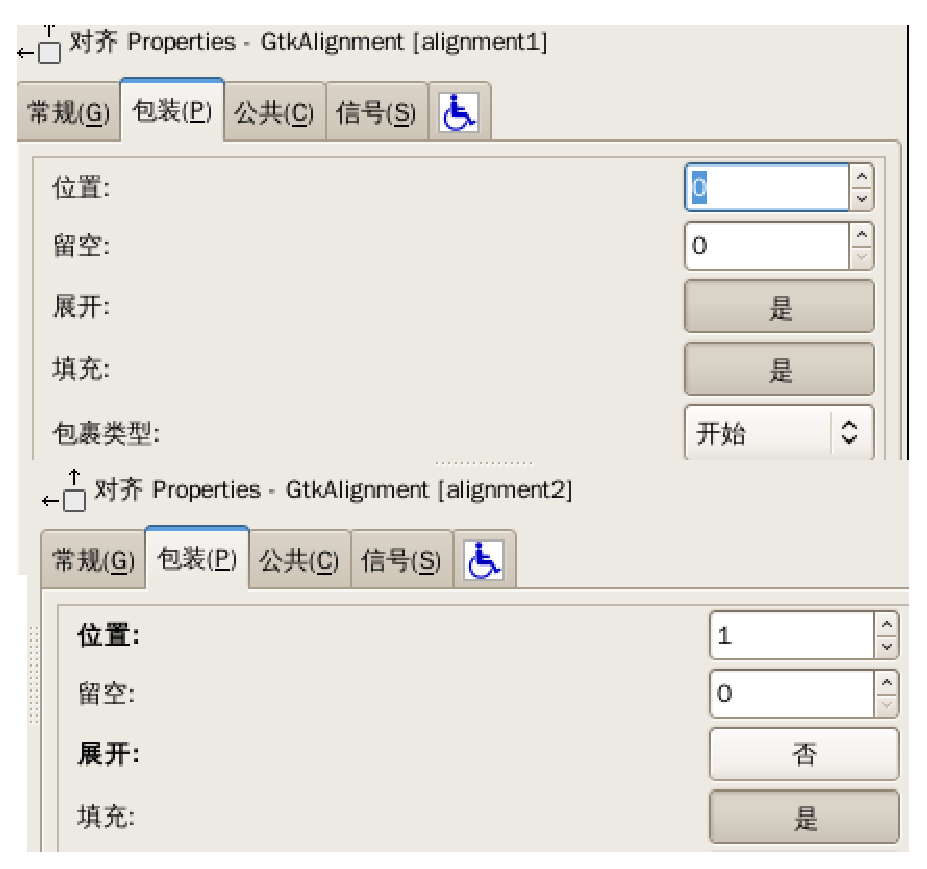
\includegraphics[width=3.5in]{images/align}
  \caption{	设置alignment}
  \label{fig:align}
\end{figure}
